%%%%%%%%%%%%%%%%%%%%%%%%%%%%%% -*- Mode: Latex -*- %%%%%%%%%%%%%%%%%%%%%%%%%%%%
%% nsf.tex         : 2009 Smart Consumer Proposal
%% Author          : Philip Johnson
%% Created On      : Tue Mar 31 11:16:58 2009
%% Last Modified By: Philip Johnson
%% Last Modified On: Thu Feb 11 08:53:51 2010
%%%%%%%%%%%%%%%%%%%%%%%%%%%%%%%%%%%%%%%%%%%%%%%%%%%%%%%%%%%%%%%%%%%%%%%%%%%%%%%
%%   Copyright (C) 2009 
%%%%%%%%%%%%%%%%%%%%%%%%%%%%%%%%%%%%%%%%%%%%%%%%%%%%%%%%%%%%%%%%%%%%%%%%%%%%%%%
%% 
 
\documentclass[11pt]{article}
\usepackage[final]{graphicx}

\usepackage[nottoc,numbib]{tocbibind}

%% Make subsubsections numbered and included in ToC
\setcounter{secnumdepth}{3}
\setcounter{tocdepth}{3}

\usepackage{multirow}

%% URLs
\usepackage{url}
\usepackage[colorlinks, bookmarks=true]{hyperref}

%% Define a new 'smallurl' style for the package that will use a smaller font.
\makeatletter
\def\url@smallurlstyle{%
  \@ifundefined{selectfont}{\def\UrlFont{\sf}}{\def\UrlFont{\small\ttfamily}}}
\makeatother
%% Now actually use the newly defined style.
\urlstyle{smallurl}

%% CO2 
\usepackage{xspace}
\newcommand{\COtwo}{CO\ensuremath{_2}\xspace}

%% Make margins less ridiculous
\usepackage{fullpage}

%% Since I'm using the LaTeX Makefile that uses dvips, I need this
%% package to make URLs break nicely
\usepackage{breakurl}

\begin{document}
\title{The Kukui Cup: \\Proposal for a UH Dorm Energy Competition}

\author{Philip M. Johnson \\
Collaborative Software Development Laboratory \\
Department of Information and Computer Sciences \\
University of Hawai'i \\
johnson@hawaii.edu \\
\url{http://csdl.ics.hawaii.edu/techreports/10-03/10-03.pdf}
}

\maketitle

\tableofcontents
\newpage

\section{Goals}

We are designing the UH Dorm Energy Competition Project (Kukui
Cup\footnote{We named the competition Kukui Cup because kukui nut oil was used by ancient Hawaiians as a source of light,
  thus serving as the earliest form of ``electricity'' in the islands.}) to achieve three goals:
\begin{enumerate}
\item Improve the {\em energy literacy} of the participating students;
\item Conduct {\em innovative, cutting edge research} in information technology for
  energy-related behavioral change;
\item {\em Save money} for the university by reducing energy costs.
\end{enumerate}

\subsection{Improve energy literacy}

Energy literacy \cite{DeWaters09b, DeWaters09} has three components:
knowledge, attitudes, and behaviors. Energy knowledge refers to factual 
information and skills, such as the ability to estimate the energy savings
in Watt-hours from switching lights from incandescent to compact
flourescent.   Energy attitudes refers to one's opinions and beliefs
related to energy, such as that conserving energy is good for
the environment.   Energy behaviors combine knowledge and attitudes to
produce concrete action, such as replacing the incandescent bulbs in one's
home with compact flourescent. 

While one might assume from the above definition that energy literate
behaviors follow naturally from knowledge and attitudes, there is
substantial research to the contrary.  For example, Geller \cite{Geller81}
performed an experiment in which 40 consumers attended a three hour
workshop on energy conservation.  A pre and post workshop questionnaire
determined that all participants gained greater awareness of energy issues,
more appreciation for what could be done in their homes to reduce energy
use and save money, and a willingness to implement the changes that were
advocated in the workshop. However, a one month followup indicated very
little actual change in behavior. One person lowered the temperature on the
hot water heater. Two additional people had installed insulating blankets
around their hot water heaters, but they had already done this before the
workshop. Finally, eight people installed low-flow shower heads---after all
40 participants had been given the low-flow shower heads at the workshop.

As this and similar research illustrates, simply providing people with
information about energy, even if it affects their attitudes, is generally
not enough to create sustained, positive behavioral change with respect to
their energy usage.  Fortunately, there is also a growing body of research
on techniques that do support behavioral change
\cite{Becker78,Darby06,Faruqui09,Houwelingen89,Peterson07,Peterson07a,Staats04,Vollink99},
which can be summarized as follows.  First, provide {\em personalized
  information} that reflects the consumer's unique circumstances.  For
example, a dorm resident will not respond well to energy tips involving
improved insulation.  Second, provide both {\em general and specific
  commitments}, especially when they can be tied to a broader issue. For
example, pledging to use a clothesline rather than a dryer because it
reduces green house gas emissions.  Third, provide {\em achievable goals}
that can be objectively measured.  An example might be to reduce energy
consumption by 10\% over the previous month.  Fourth, elicit {\em social
  reinforcement} which can be manifested in both overt and subtle ways.
For example, in dorm settings, as more and more residents publicly
participate, it implicitly becomes ``the thing to do''.  Fifth, provide
{\em constant and contextual feedback} which helps verify progress toward
goals and can reinvigorate commitments, as long as the feedback is provided
in the right way at the right time.  Sixth, {\em financial incentives} can
be a powerful motivator for energy conservation. For example, a prize such
as iPods to the members of the dorm floor who conserved the most energy.

Thus, the first design goal of the dorm energy competition is to increase
factual knowledge about energy by participants, foster more sophisticated
attitudes based upon this knowledge, and, most finally, facilitate actual
behavioral change.


\subsection{Conduct innovative IT energy research}

As noted in the previous section, there is evidence in support of a variety
of techniques for promoting sustained, positive behavioral change, but
current dorm energy competitions either do not employ these techniques, or
they do not utilize information technology effectively to deploy the
techniques or support assessment of their effectiveness.

The most common form of information technology support for dorm energy
competitions is a simple relatively static web site, as illustrated in
Figure \ref{fig:wellesley}.  These websites provide access to resources
about energy, and feedback regarding energy usage for the entire building
every few days.  The most sophisticated technology to date is the Campus
Resource Monitoring System at Oberlin College, which has the potential to
provide near-real time energy consumption data\footnote{With respect to
  energy consumption data, we define ``near-real time'' as sub-minute
  update intervals.  For example, obtaining meter data every 10 seconds is
  ``near real time'', while obtaining meter data every 15 minutes is not.}.

\begin{figure*}[!ht]
  \center
  \includegraphics[width=0.8\textwidth]{wellesley.ppt.eps}
  \caption{\em \small The Wellesley College Dorm Energy Competition Web site.}
 \label{fig:wellesley}
\end{figure*} 


We are designing a collection of software services that will provide UH
dorm residents participating in the competition with unparalleled
information technology support for improving their energy literacy.  Our
software will support a unique combination of features including: (a)
near-real time energy consumption data, (b) floor-level as well as
building-level energy data; (c) personalized, login-protected pages for
each student; (d) energy literacy activities with a ``Kukui Nut'' award
system for participation; and (e) integration with other information
technologies used by students, including text messaging, Facebook, email,
and Twitter.

Our software services are not designed merely to be cool or trendy; they
are designed to enable substantial, important research into energy
behavior. While prior research has generated evidence regarding a variety
of techniques for fostering behavioral change, there is relatively little
understanding of the relative importance or impact of these methods.  Our
software will enable us to present students with a variety of avenues for
participation and determine the ways in which they took part. It will also
enable us to observe and record their energy usage (on a floor-by-floor
basis) before, during, and after the competition.  In addition, we will
request student volunteers for an energy literacy assessment both before
and after the competition.  The result of these three streams of data will
provide a uniquely rich source of insight into the popularity of various
activities, their impact on energy literacy, and the final impact on actual
energy usage.  

More details on the software are provided below, but in summary, the goal
of our software is to provide innovative support for improving energy
literacy in students combined with infrastructure to enable ground-breaking
empirical research in sustainability and energy.

\subsection{Save money}

The final goal is to save money.  Previous dorm energy challenges at
Brandeis University, Carleton College, Harvard University, MIT, Mount
Holyoke College, Ohio University, and Williams College have reported energy
savings, generally in the range of 7\% to 16\%.  If we can achieve these
results, and if the savings can be sustained for the remainder of the
school year, then energy costs for the dorms alone could be reduced by tens
of thousands of dollars.

However, those are just the ``first-order'' savings to the university.  If
the competition achieves the goal of improving the energy literacy of
students, then their energy literate behavior will be manifested everywhere
on campus, not just in their dorm floors.  A more energy literate student
will choose energy saving behaviors in campus cafeterias, classrooms, and
labs, producing additional, ``second-order'' savings to the university.
Furthermore, the ``return on investment'' in improved energy literacy will
occur over their entire time at the university, not just during the one
month competition, and not just during their one year in the dorm.  We also
hope that these energy literate students will influence their friends in
positive ways, reaping additional dividends.

There is even the possibility of ``third-order'' savings.  We are designing
this project to begin with dormitory energy competitions, then extend into
residential community energy challenges \cite{csdl2-09-15}.  In addition,
we are releasing all software developed under this project as open source
in order to facilitate more wide-spread adoption.  Thus, this project could
lead to eventual energy cost savings in our community and elsewhere.

\section{Approach}

\subsection{Design components}

\subsection{Architecture}

\subsection{User Interface}

\subsection{Meters}

\subsection{Contents}

\subsection{Timeline}

\subsection{Stakeholders}


\section{Final thoughts: Why care about behavior?}

There is a school of thought that views human behavior as too difficult to
change and ultimately unreliable, and that the only realistic approach to
energy conservation is through ``top-down'' incorporation of new technology
that eliminates the need for human decision-making/behavior.  For example,
to reduce energy in the dorm, the best approach is to have the Housing
Office and Facilities Management improve the efficiency of air
conditioning, replace the light bulbs, increase the amount of insulation,
and so forth.

We certainly agree that the introduction of new technology is desirable and
should be done whenever possible.  Indeed, a study by Granade \cite{Granade09}
shows that U.S. energy consumption could be reduced by almost 25\% if
cost-effective energy saving technology already available was implemented.

However, we disagree that behavior is too difficult or leads to only
marginal results.  An old, inefficient air conditioner uses far less energy
than a state-of-the-art unit if an energy literate student decides to turn
it off (or not turn it on at all).  The energy associated with landfill
management is reduced when an energy literate student chooses a
non-styrofoam container, or to bring their own bag to the farmers market.

Finally, we disagree that ``top-down'' approaches are the only viable way
to effect conservation-related change, and suggest that the rapidly growing
organic foods industry provides a compelling example.  There was no
top-down mandate for organic foods in this country. Rather, a growing
number of ``food-literate'' consumers began buying these foods despite
their generally higher price.  The result is annual industry growth of over
20\% for the past several years.  We believe that energy literacy can
catalyze a similar appetite for energy conservation.







\bibliography{smartconsumer,csdl-trs}
\bibliographystyle{plain}
\end{document}
